\begin{enumerate}

%-------- ejercicio 4
\item Demuestre vectorialmente y euclidianamente la siguinetes propiedad.\\
Los puntos medios de dos lados de un triángulo forman un segmento paralelo al tercer lado cuya longitud es la mitad de la longitud del tercer lado.\\\\
    Demostración.-\;
    \begin{center} 
	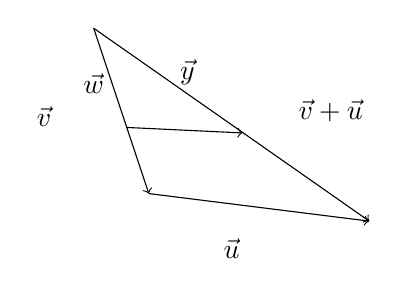
\begin{tikzpicture}[scale=.7]
	   \draw[->](0,0)--(4,-.5); 
	   \draw(-1.9,1.4)node[]{$\vec{v}$};
	   \draw(-1,2)node[]{$\vec{w}$};
	   \draw[<-](0,0)--(-1,3);
	   \draw(1.5,-1)node[]{$\vec{u}$};
	   \draw[->](-1,3)--(4,-.5);
	   \draw(3.3,1.5)node[]{$\vec{v}+\vec{u}$};
	   \draw[->](-.4,1.2)--(1.7,1.1);
	   \draw(.7,2.2)node[]{$\vec{y}$};
	\end{tikzpicture}
    \end{center} 
    Sea $\vec{v}$, $\vec{u} \in V_n$ dos lado del triángulo, de donde el tercer lado está formado por $\vec{v}+\vec{u}$. Luego por hipótesis $$\vec{v}=2\vec{w}\quad \mbox{y}\quad \vec{v}+\vec{u} = 2\vec{y} \qquad \mbox{para}\; w,y\in V_n.$$ 
    En consecuencia $$\vec{u}=2(\vec{w}-\vec{y})$$
    por lo tanto por definición de vectores paralelos se demuestra la proposición requerida.\\\\

\end{enumerate}
